In this section an alloy formulation is provided to model critical aspects of the system. The analysis is mainly focused on the satisfiability of some static constraints, in particular:
\begin{itemize}
	\item it cannot happen that two different users have the same email address.
	\item each city must have at most one municipality, and a municipality is associated to only one city.
	\item authorities have the jurisdiction of only one city, but a city can have multiple registered authorities.
	\item data requests must satisfy the filters.
	\item requested data must be compliant with the user authorization.
\end{itemize}

\vspace{10mm}
\lstinputlisting[language=alloy]{Alloy/Model.als}


\begin{figure}[H]
	\centering
	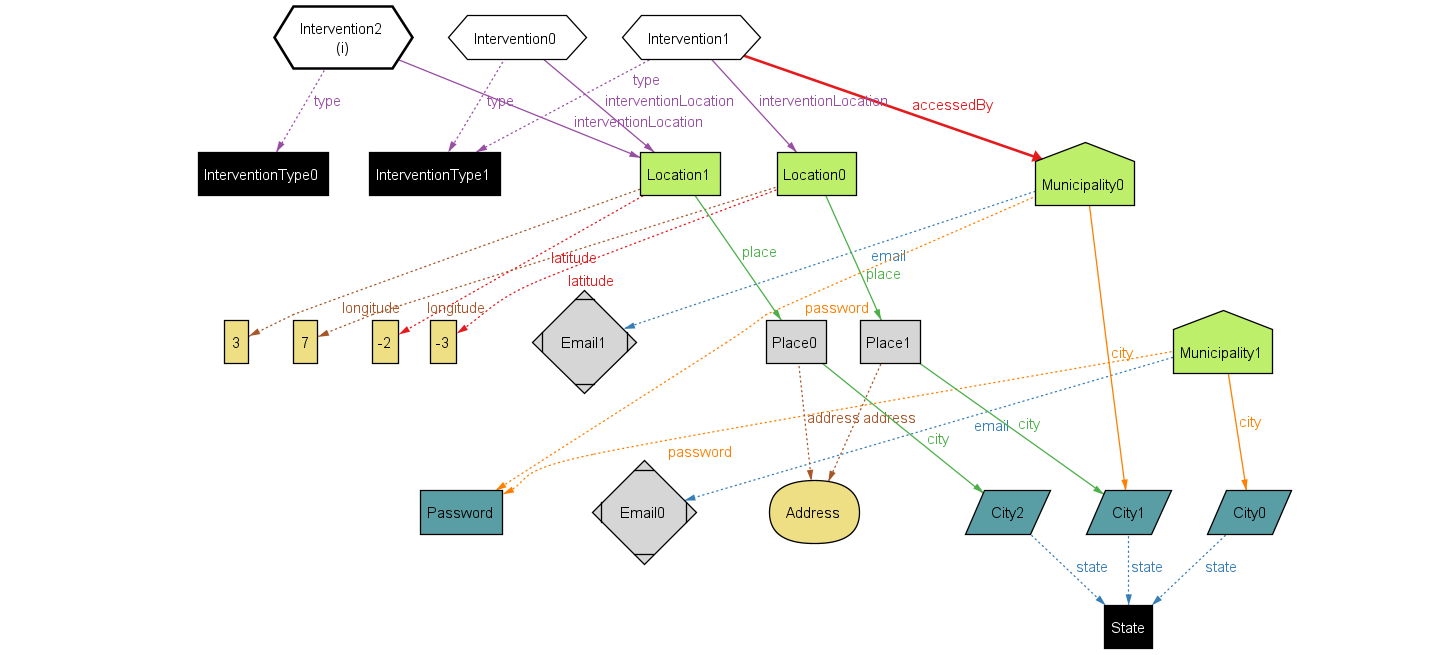
\includegraphics[width=\textwidth]{Alloy/interventionAccessibility}
	\caption{World 3}
\end{figure}

From world 3 we can check that an intervention can be seen only by municipality of the city in which the intervention is situated, otherwise the intervention exists but can't be visualized by any municipality. Generating interventions for non registered municipalities can be useful because any municipality that register to the service can visualize a list of interventions right away, so we have allowed this case.

\begin{figure}[H]
	\centering
	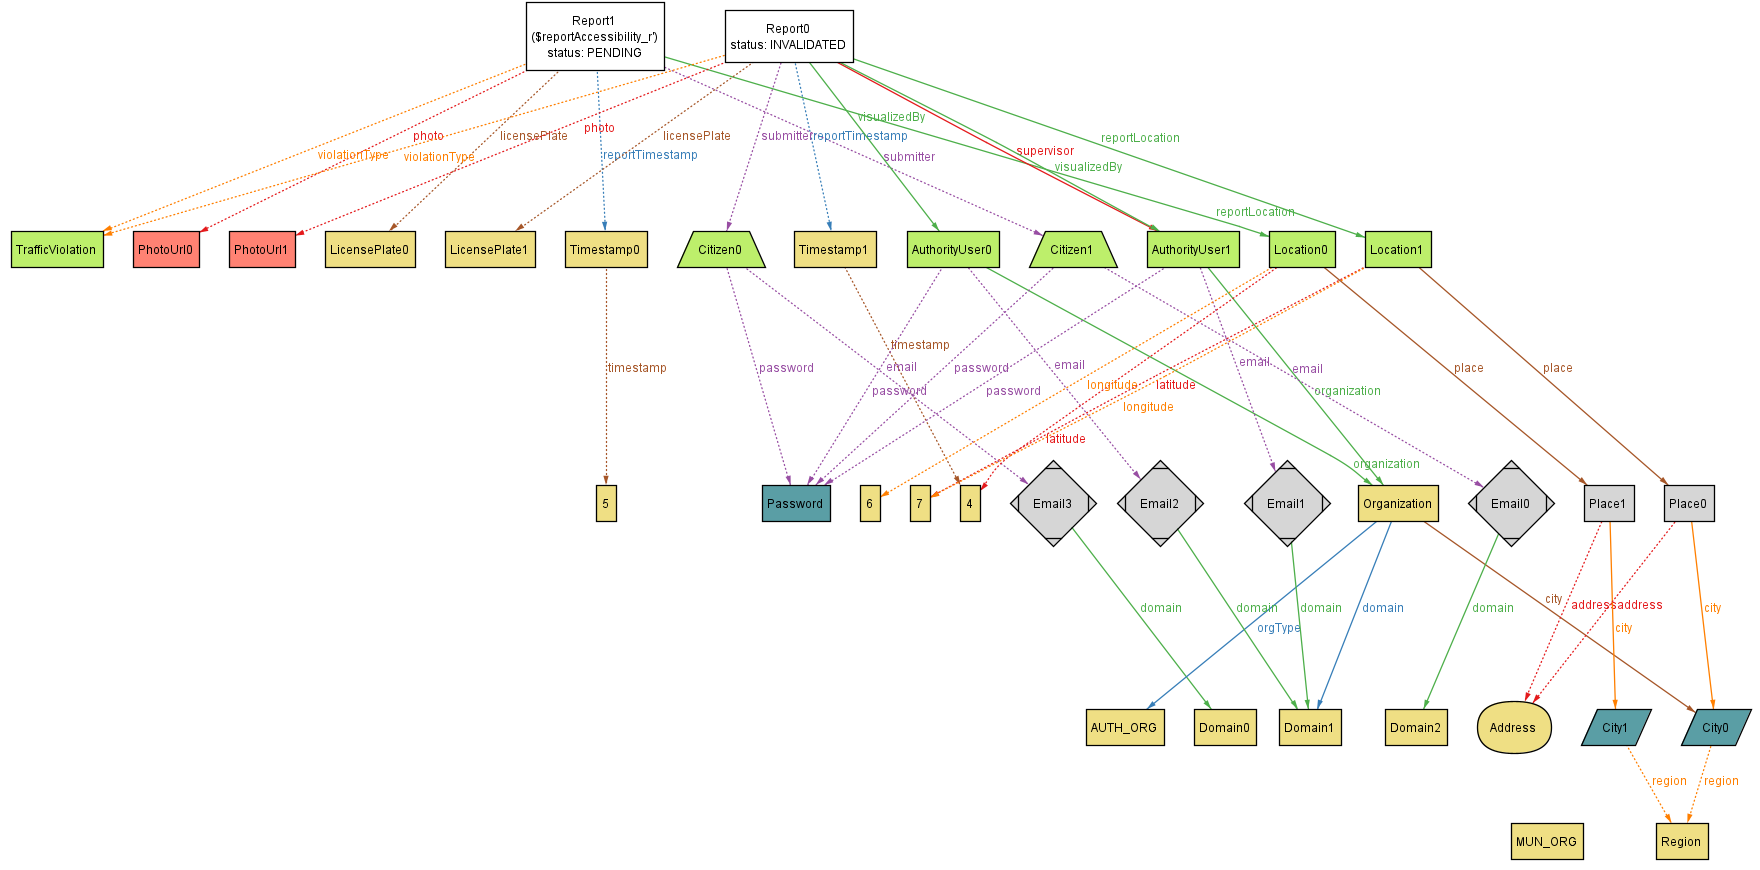
\includegraphics[width=\textwidth]{Alloy/reportAccessibility}
	\caption{World 4}
\end{figure}

From world 4 we can check that a report can be visualized only by authorities who have jurisdiction on that city. Another interesting relation is that report supervisor is of course an authority that can access it, also if a supervisor is present means that report is either validated or invalidated. If a report can't be accessed, clearly its status remain always pending because no authority can't change it.